A triangle's {\em Inconic} touches its three sides while satisfying two other constraints, e.g., the location of its center. Similar to Circumconics, if the latter is interior to the 4 shaded regions in  Figure~\ref{fig:midlines} it is an ellipse, else it is a hyperbola. Lines drawn from each vertex to the Inconic tangency points concur at the perspector or Brianchon Point $B$ \cite{mw}.

Let the Inconic center $C$ be specified by Barycentrics\footnote{Barycentrics $g$ can be easily converted to Trilinears $f$ via: $f(s_1,s_2,s_3)=g(s_1,s_2,s_3)/s_1$ (cyclic) \cite{yiu2003}.} $g(s_1,s_2,s_3)$ (cyclic), then $B$ is given by $1/[g(s_2,s_3,s_1)+g(s_3,s_1,s_2)-g(s_1,s_2,s_3)]$ (cyclic) \cite{stothers2001-circumconics}. For example, consider the Inconic centered on $X_1$ (the Incircle), i.e., $g=s_2 s_3$ (cyclic). Then $B=1/(s_1 s_3+s_1 s_2-s_2 s_3)$. Dividing by the product ${s_1}{s_2}{s_3}$ obtain $B=1/(s_2 + s_3 - s_1)$ (cyclic), confirming that the perspector of the Incircle is the Gergonne Point $X_7$ \cite[Perspector]{mw}. The contact points are the vertices of the Cevian triangle through $B$.

Above we identified the confocal Caustic with the Mandart Inellipse $I_9$ \cite{mw} of the 3-periodic family, i.e., it is a stationary ellipse centered on $X_9$ and axis-aligned with the EB, Figure~\ref{fig:three-orbits-proof}. Its semi-axes $a_c,b_c$ are given by \cite{garcia2019-incenter}:

\begin{equation*}
a_c=\frac{a\left(\delta-{b}^{2}\right)}{a^2-b^2},\;\;\;
b_c=\frac{b\left({a}^{2}-\delta\right)}{a^2-b^2}\cdot
\end{equation*}

Similarly, the $X_9$-centered Inconic of the family of Excentral Triangles is the stationary EB, i.e., the EB is the Orthic Inconic \cite{mw} of the Excentrals.

\subsection{Excentral X$_3$-Centered Inconic}

No particular invariants have yet been found for any of the Inconics to 3-periodics with centers in $X_i$, $i=3,4,\ldots,12$. Let $I_3$ denote the $X_3$-centered inconic. Its Brianchon Point is $X_{69}$ and its foci aren't named centers \cite{moses2020-private-circumconic}.

\begin{remark}
$I_3$ is always an ellipse.
\end{remark}

To see this consider the Circumcenter of an acute, right, or obtuse triangle lies inside, on a vertex, or opposite to the interior of the Medial, respectively, i.e., within one of the 4 shaded regions in Figure~\ref{fig:midlines}.

Let $I'_3$ denote the $X_3$-centered Inconic of the Excentral Triangle. Its Brianchon Point is $X_{69}$ of the Excentral, i.e., $X_{2951}$ of the reference 3-periodic \cite{moses2020-private-circumconic}, Figure~\ref{fig:macbeath-excentral}(left).

\begin{remark}
$I'_3$ is axis-aligned with the EB and intersects it at $X_{100}$.
\end{remark}

\noindent Let $\mu'_3,\mu_3$ denote $I_3'$ major and minor semi-axes.

\begin{conjecture}
$\mu_3'/\mu_3$ is invariant over all 3-periodics and given by:

\begin{equation*}
\frac{\mu_3'}{\mu_3}=
%\frac{\sqrt{2\delta(\delta+ a^2 - b^2) - a^2 b^2}}{b^2} =
\frac{R+d}{R-d} = \frac{1+\sqrt{1-2\rho}}{\rho}-1
\end{equation*}
\label{conj:excIncX3}
\end{conjecture}

\noindent with $d=\sqrt{R(R-2r)}$, and $\rho=r/R$. The above has been derived for an isosceles 3-periodic. It matches the ratio numerically for any combination of $a,b$.

\subsection{Excentral  X$_5$-Centered (MacBeath) Inconic}

Above the locus of the Excenters is identified with the Excentral MacBeath Circumconic $E_6' $. The MacBeath {\em Inconic} $I_5$ of a triangle is centered on $X_5$ and has foci on $X_4$ and $X_3$. Its Brianchon Point is $X_{264}$, and it can be both an ellipse or a hyperbola \cite[MacBeath Inconic]{mw}. No invariants have yet been found for $I_5$.

Consider $I'_5$, the MacBeath Inconic of the Excentral Triangle, Figure~\ref{fig:macbeath-excentral}(right). The center and foci of $I'_5$ with respect to the reference triangle are $X_3$, $X_1$, and $X_{40}$, respectively, and its Brianchon is $X_{1742}$ \cite{moses2020-private-circumconic}. Unlike $I'_3$, the axes of $I'_5$ are askew with respect to the EB.

\begin{remark}
$I'_5$ is always an ellipse.
\end{remark}

This is due to the fact that the Excentral is acute as is its homothetic Medial. Since $X_5$ is the latter's Circumcenter, it must lie inside it.

\noindent Let $\mu'_5,\mu_5$ denote $I_5'$ major and minor semi-axes.

\begin{conjecture}
$\mu_5'/\mu_5$ is invariant over all 3-periodics and given by:

\begin{align*}
 \frac{\mu'_5}{\mu_5} =
 %\frac {\left( {b}^{2}+\delta \right) \sqrt {\delta+{a}^{2}-{b}^{2} } }{2b{a}^{2}}=
 %\frac {\left( {a}^{2}+\delta \right) \sqrt {\delta+{b}^{2}-{a}^{2}} }{2a{b}^{2}} =
\frac{R}{\sqrt{R^2-d^2}}=\frac{1}{\sqrt{2 \rho}}
\end{align*}
\label{conj:excIncX5}
\end{conjecture}

The above was derived for an isosceles 3-periodic and shown to work for any $a,b$.

\begin{figure}
    \centering
    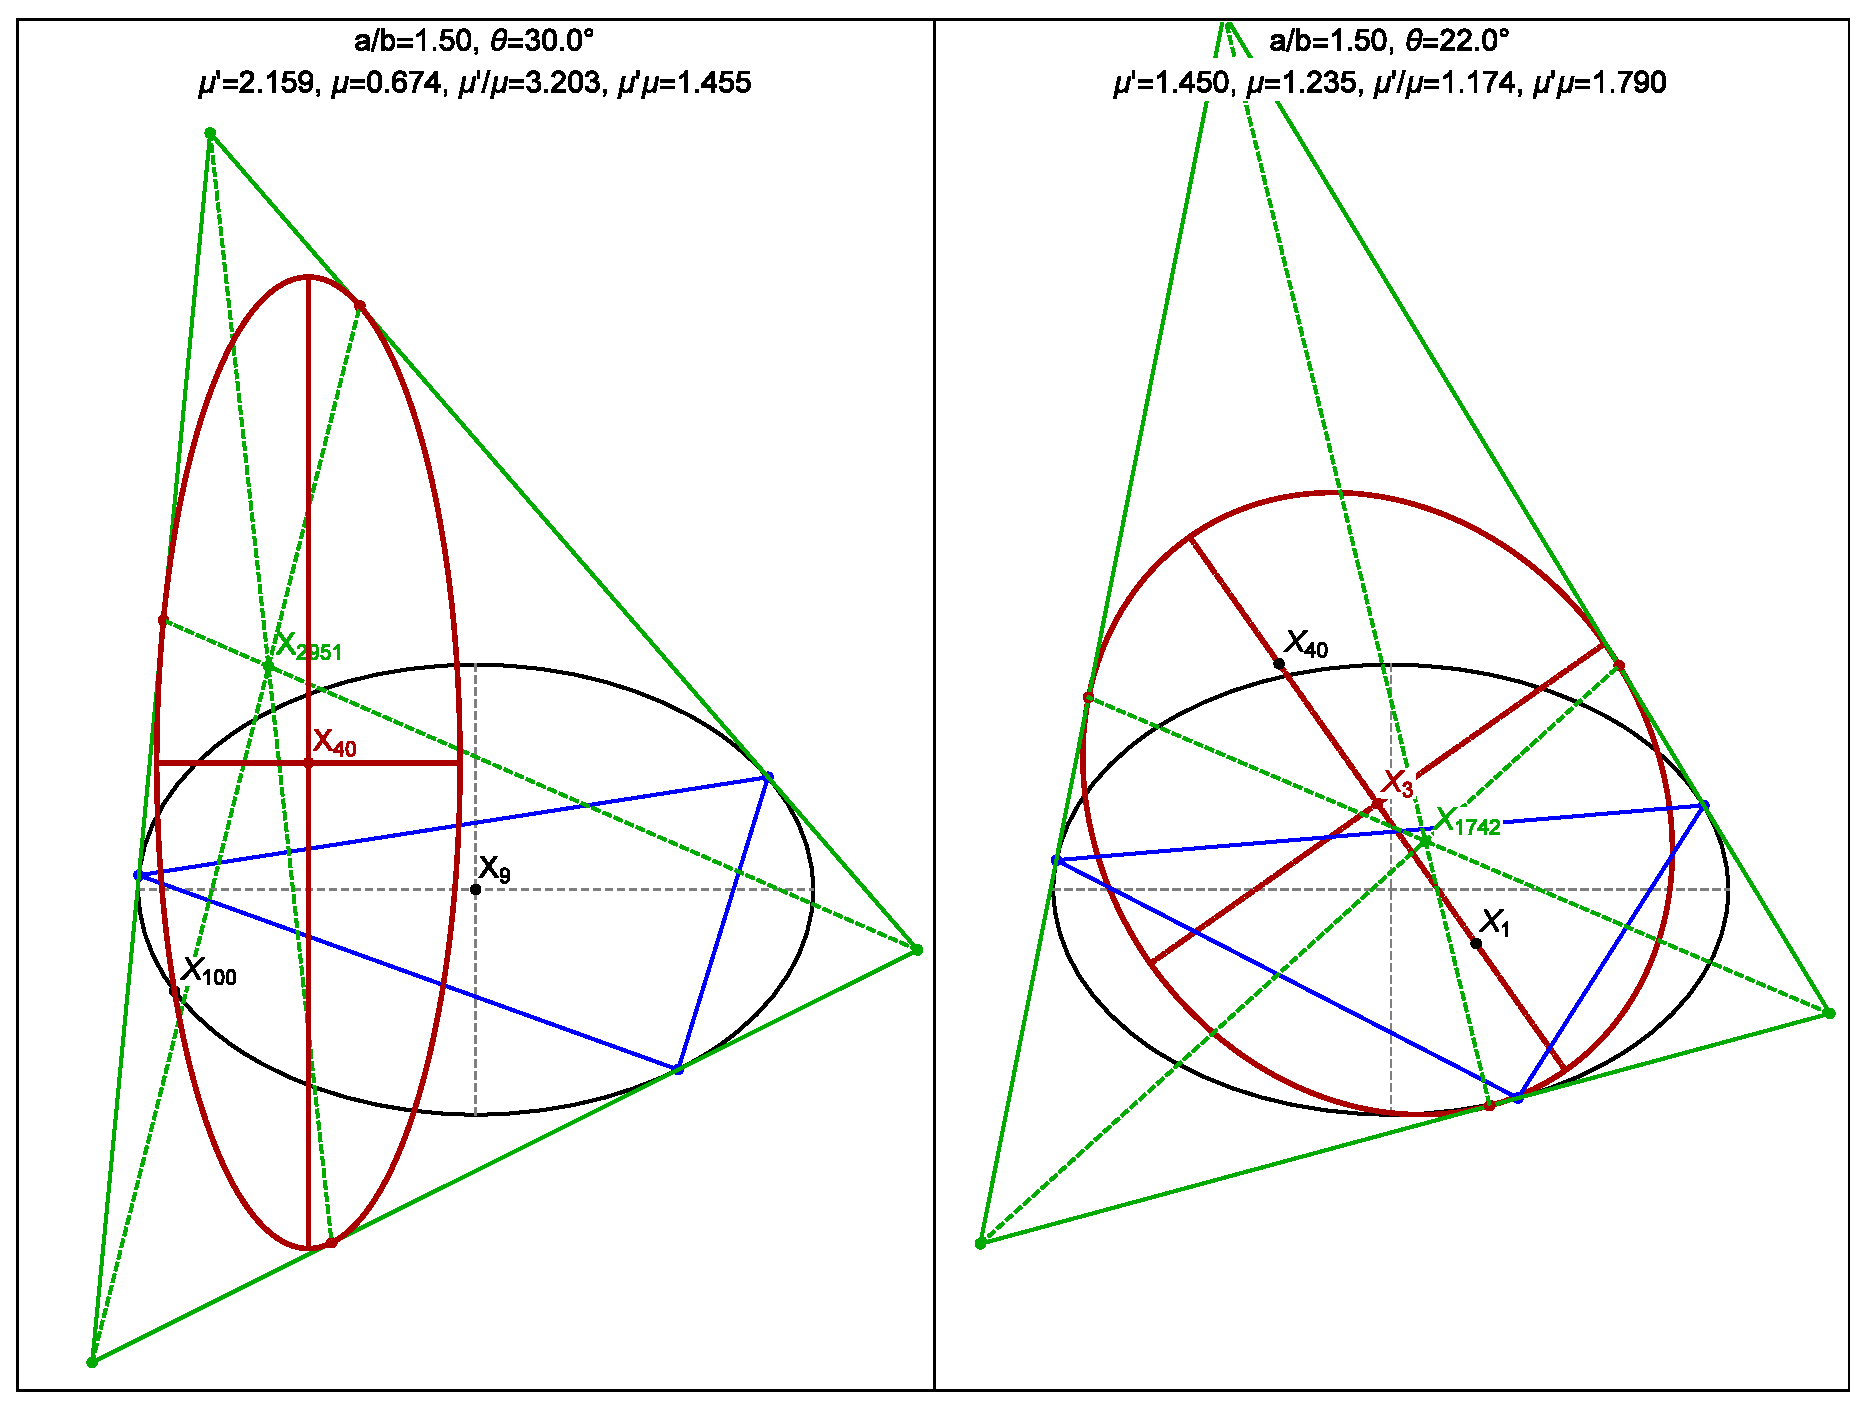
\includegraphics[width=\textwidth]{pics_eps_new/0150_two_inconics.eps}
    \caption{\textbf{Left}: The $X_{3}$-centered Inconic (red) of the Excentral Triangle (green), whose center is $X_{40}$ in terms of the 3-periodic (blue). Its Brianchon Point is $X_{2951}$ \cite{moses2020-private-circumconic}. This Inconic's axes are aligned with the EB which it intersects at $X_{100}$, and its aspect ratio is invariant. \textbf{Right}: The MacBeath Inconic of the Excentral (red) is centered on the latter's $X_5$ and has foci on $X_4$ and $X_3$. These correspond to  $X_3$, $X_1$, and $X_{40}$ of the reference triangle (blue). Its Brianchon Point is $X_{1742}$ \cite{moses2020-private-circumconic}. Though its axes are askew with respect to the EB, its aspect ratio is invariant over the 3-periodic family. \textbf{Video}: \cite[PL\#11]{reznik2020-playlist-circum}.}
    \label{fig:macbeath-excentral}
\end{figure}